\pdfminorversion=4
\documentclass[9pt]{beamer} 
\setbeamertemplate{navigation symbols}{}
%\setbeamertemplate{frametitle}{}

%\usetheme{Montpellier}
%\setbeamertemplate{footline}[frame number]

\usepackage{pgfpages}
\usepackage{booktabs}
\usepackage[%				
%   group-separator = {.}, 			 % group-seperator={,} -> 1,345,234.23
%   round-mode 		= places,		 % round-mode= places(2digits), figures(1digit)
%   round-precision = 3,			 % round-precision= x , xdigits are rounded to
	binary-units 	= true,			 % Laden von \byte \bit, \kibi usw. (false default)
	locale = DE,					 % lacale= DE, uses german
	per=slash,
%	loctolang={UK:english, DE:ngerman},	% loctolang={USA:USenglish,DE:ngerman}, if language changed in
									 % document
%			detect-all,				 % detect-all : uses the text options not the math mode to set
									 % the letters/numbers
			]{siunitx}				 % For typical Units in Text- and Mathmode
%%%%%%%%%%%%%%%%%%%%%%%%%%%%%%%%%%%%%%%
% Loading mathematical writing style  %
%%%%%%%%%%%%%%%%%%%%%%%%%%%%%%%%%%%%%%%
\usepackage{mathtools}
    
\mode<presentation>
{
%\usetheme{Madrid}
\usetheme{Boadilla}

\setbeamercovered{transparent}
}
\usepackage{subfigure} 
\usepackage{amsmath}  			% erleichtert Mathe 
\usepackage{enumerate}			% schicke Nummerierung
\usepackage{graphicx} 			% für Grafik-Einbindung
\usepackage{multicol}
\usepackage{lmodern}
\usepackage[ngerman]{babel}
\usepackage[utf8]{inputenc}

\usepackage{listings}
\lstset{ %
  backgroundcolor=\color{white},   % choose the background color; you must add \usepackage{color} or \usepackage{xcolor}; should come as last argument
  basicstyle=\footnotesize,        % the size of the fonts that are used for the code
  breakatwhitespace=false,         % sets if automatic breaks should only happen at whitespace
  breaklines=true,                 % sets automatic line breaking
  captionpos=b,                    % sets the caption-position to bottom
  commentstyle=\color{mygreen},    % comment style
  deletekeywords={...},            % if you want to delete keywords from the given language
  escapeinside={\%*}{*)},          % if you want to add LaTeX within your code
  extendedchars=true,              % lets you use non-ASCII characters; for 8-bits encodings only, does not work with UTF-8
  frame=single,	                   % adds a frame around the code
  keepspaces=true,                 % keeps spaces in text, useful for keeping indentation of code (possibly needs columns=flexible)
  keywordstyle=\color{blue},       % keyword style
  language=Matlab,                 % the language of the code
  morekeywords={*,...},            % if you want to add more keywords to the set
  numbers=left,                    % where to put the line-numbers; possible values are (none, left, right)
  numbersep=5pt,                   % how far the line-numbers are from the code
  numberstyle=\tiny\color{mygray}, % the style that is used for the line-numbers
  rulecolor=\color{black},         % if not set, the frame-color may be changed on line-breaks within not-black text (e.g. comments (green here))
  showspaces=false,                % show spaces everywhere adding particular underscores; it overrides 'showstringspaces'
  showstringspaces=false,          % underline spaces within strings only
  showtabs=false,                  % show tabs within strings adding particular underscores
  stepnumber=2,                    % the step between two line-numbers. If it's 1, each line will be numbered
  stringstyle=\color{mymauve},     % string literal style
  tabsize=2,	                   % sets default tabsize to 2 spaces
  title=\lstname                   % show the filename of files included with \lstinputlisting; also try caption instead of title
}

\usepackage{media9}
%\usepackage{multimedia}

%=================== Set Beamer Templates ====================================
%\definecolor{DOGGYbg}{RGB}{167,183,208} %HAW Color 
%\definecolor{DOGGY}{RGB}{26,60,116} % HAW Color 2
%\definecolor{DOGGYbg}{RGB}{240,240,255} %HAW Color 
%\definecolor{DOGGY}{RGB}{26,60,116} % HAW Color 2
%\definecolor{dgreen}{RGB}{0,150,0} % HAW Color 2
%\definecolor{lightgray}{RGB}{150,150,150} % HAW Color 2

%\setbeamercolor*{structure}{fg=DOGGY, bg=DOGGYbg}
%\setbeamercolor*{palette primary}{use=structure,fg=structure.bg,bg=structure.fg!95!black}
%\setbeamercolor*{palette secondary}{use=structure,fg=structure.bg,bg=structure.fg!70!black}
%\setbeamercolor*{palette tertiary}{use=structure,fg=structure.bg,bg=structure.fg!95!black}
%\setbeamercolor*{palette quaternary}{fg=structure.bg,bg=black}
%\setbeamercolor*{block title}{use=structure,fg=structure.bg,bg=structure.fg!75!black}

\definecolor{DOGGYbg}{RGB}{80,90,100} %HAW Color
\definecolor{DOGGY}{RGB}{26,60,116} % HAW Color 2
\definecolor{lgray}{RGB}{240,240,240} %HAW Color
\definecolor{darkgreen}{RGB}{50,150,50} %HAW Color

\definecolor{mygreen}{rgb}{0,0.6,0}
\definecolor{mygray}{rgb}{0.5,0.5,0.5}
\definecolor{mymauve}{rgb}{0.58,0,0.82}

\setbeamercolor*{structure}{fg=DOGGY, bg=DOGGYbg} 
\setbeamercolor*{palette primary}{use=structure,fg=structure.fg,bg=lgray}
\setbeamercolor*{palette secondary}{use=structure,fg=structure.fg,bg=lgray!90!black}
\setbeamercolor*{palette tertiary}{use=structure,fg=structure.fg,bg=lgray}
\setbeamercolor*{palette quaternary}{fg=structure.fg,bg=lgray}
\setbeamercolor*{block title}{use=structure,fg=structure.fg,bg=lgray}


\setbeamertemplate{navigation symbols}{} % No navigation symbols
\setbeamercolor{navigation symbols}{use=structure, fg=structure.bg,
bg=structure.bg}
% New footline
\defbeamertemplate{footline}{rownav}{%
  \leavevmode%
  \hbox{%
  \begin{beamercolorbox}[wd=.15\paperwidth,ht=2.5ex,dp=1ex,center]{author in
  head/foot}% only put the author and dont use the institute name - width 1/4
    \usebeamerfont{author in head/foot}\insertshortauthor
  \end{beamercolorbox}%
  \begin{beamercolorbox}[wd=.60\paperwidth,ht=2.5ex,dp=1ex,center]{title in
  head/foot}%
    \usebeamerfont{title in head/foot}\insertshorttitle
  \end{beamercolorbox}%
  \begin{beamercolorbox}[wd=.08\paperwidth,ht=2.5ex,dp=1ex,right]{date in
  head/foot}%
    \usebeamercolor[fg]{navigation symbols}% 
    \insertslidenavigationsymbol\hspace*{1ex}%
    \vspace*{-0.5ex}
  \end{beamercolorbox}%
  \begin{beamercolorbox}[wd=.17\paperwidth,ht=2.5ex,dp=1ex,center]{date in
  head/foot}%
    \usebeamerfont{date in head/foot}\insertshortdate{}\hspace*{2em}
    \textbf{\insertframenumber{}}% 
  \end{beamercolorbox}%
    }%
  \vskip0pt%
}
\setbeamertemplate{footline}[rownav]{}

\defbeamertemplate*{title page}{myPage}[1][]
{
  \vbox{}
  \vfill
  \begin{centering}
    \begin{beamercolorbox}[sep=8pt,center,#1]{author}
      \usebeamerfont{title}\inserttitle
    \end{beamercolorbox}%
    \vskip1em\par
    \begin{beamercolorbox}[sep=8pt,center,#1]{author}
      \usebeamerfont{author}\insertauthor
    \end{beamercolorbox}
    \begin{beamercolorbox}[sep=8pt,center,#1]{institute}
      \usebeamerfont{institute}\insertinstitute
    \end{beamercolorbox}
    \begin{beamercolorbox}[sep=8pt,center,#1]{date}
      \usebeamerfont{date}\insertdate
    \end{beamercolorbox}
  \end{centering}
  \vfill
}
 
\setbeamertemplate{title page}[myPage]{}
% ============== Document begin ==============================================


%=====================================================================================%
%	Titel und Authoren auf der ersten Seite
%=====================================================================================%
\title[Diskretisierungsfehler der Twiddlefaktoren]{\textbf{ISAR -- Projektmeeting}\\ 
\medskip Abweichungen von Twiddlefaktoren\\ als duale Festkommazahlen im SQ12-Format \\ von ihrer dezimalen Darstellung}  

\author[TL]{Thomas Lattmann}
\date[\today]{\today} 
%-----------------------------------------------------------------------------------------------
\renewcommand*{\thesubfigure}{}
\newcommand{\vid}[2]{\movie[width=.9\textwidth,height=0.9\textheight,loop,showcontrols]{\includegraphics[width=.9\textwidth,height=0.9\textheight]{#1}}{#2}}
\newcommand{\mytitle}[1]{\begin{block}{}\begin{center}#1\end{center}\end{block}}
\newcommand{\figh}[2]{\begin{figure}\centering \includegraphics[height=#1\textheight]{#2}\end{figure}}
\newcommand{\figw}[2]{\begin{figure}\centering \includegraphics[width=#1\textwidth]{#2}\end{figure}}
\newcommand{\fighw}[4]{\begin{figure}\centering\caption{#4} \includegraphics[height=#1\textheight,width=#2\textwidth]{#3}\end{figure}}
\newcommand{\fig}[1]{\begin{figure}\centering \includegraphics[scale=1]{#1}\end{figure}}
\newcommand{\bull}[1]{\begin{itemize}\item #1 \end{itemize}}
\usepackage{nameref} 
\newcommand{\cmk}{\textcolor{green}{\large\checkmark}}
\newcommand{\mtx}[1]{\ensuremath{\boldsymbol{{\mathrm{#1}}}}}
\newcommand*\colvec[3][]{\begin{pmatrix}\ifx\relax#1\relax\else#1\\\fi#2\\#3\end{pmatrix}}
%-----------------------------------------------------------------------------------------------
% 	Coloums 
%-----------------------------------------------------------------------------------------------
\newcommand{\cols}[4]{ \begin{columns} \column[T]{#1\textwidth} #3 \column[T]{#2\textwidth} #4 \end{columns}}
\newcommand{\colss}[4]{ \begin{columns} \column{#1\textwidth} #3 \column{#2\textwidth} #4 \end{columns}}
%-----------------------------------------------------------------------------------------------
\begin{document}

%==================================================================================================================================
% 	Titelseite mit Thema der Arbeit, Author und Einleitung geben, was das Hautziel ist! 
%==================================================================================================================================
%%%%%%%%%%%%%%%%%%%%%%%%%%%%%%%%%%%%%%%%%%%%%%%%%%%%%%%%%%%%%%%%%%%%%
% Define a background image for the first page
%%%%%%%%%%%%%%%%%%%%%%%%%%%%%%%%%%%%%%%%%%%%%%%%%%%%%%%%%%%%%%%%%%%%%
%\usebackgroundtemplate{\includegraphics[]{backT.pdf}}
\usebackgroundtemplate{}
\begin{frame}[plain]
	\titlepage
	\hfill
	\begin{center}
		\figw{.3}{Einstellungen/hawlogo.pdf}
	\end{center}
\end{frame}

\usebackgroundtemplate{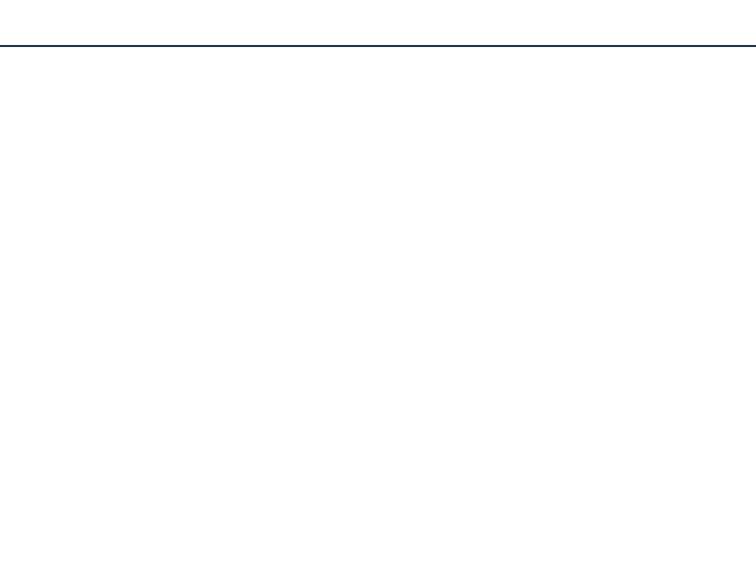
\includegraphics[scale=1]{Einstellungen/back.pdf}}
%=============================================================================
	%\begin{frame}\frametitle{Inhalt}
	%	\tableofcontents
	%\end{frame}	

%=============================================================================
	\begin{frame}\frametitle{Matrizenvergleich}

	\begin{table}\caption{Vergleich von verschiedenen DFT-Matrizen}
	  \begin{tabular}{ccccl}
	    \toprule
	    N & NxN $\cdot$ 2 & ``gute'' Werte & ``schlechte'' Werte & Verhältnis\\
	    \midrule
	    4  & 32  & 32  &   0 & Inf\\
	    8  & 128 & 96  &  32 & 3\\
	    9  & 162 & 66  &  96 & 0.6875\\
	    12 & 288 & 224 &  64 & 3.5\\
	    15 & 450 & 126 & 324 & 0.389\\
	    16 & 512 & 256 & 256 & 1\\
	    \bottomrule
	  \end{tabular}
	 \end{table}

	 
	\end{frame}
	
%=============================================================================
	\begin{frame}\frametitle{8x8 Matrix}
		\begin{table}[ht]\caption{``schlechte'' Twiddlefaktoren der 8x8 Matrix, real \& imag}
		 \begin{tabular}{rrr}
		  \toprule
		  Dezimalzahl & dezimale Darstellung der Binärzahl & prozentuale Abweichung\\
		  \midrule
		  -0.707110   & -0.707520  & 0.057916\\
		   0.707110   &  0.707031  & 0.011137\\
		   \bottomrule
		 \end{tabular}\label{8x8Matrix}
		\end{table}

			
		%\figw{0.7}{IMG/AnwendungISAR.pdf}{\tiny Darstellung von Schüthe}	
	\end{frame}
%=============================================================================
	\begin{frame}[t]\frametitle{9x9 Matrix}
	
		\begin{table}[ht]\caption{``schlechte'' Twiddlefaktoren der 9x9 Matrix, real \& imag}
		 \begin{tabular}{rrr}
		 \toprule
		  Dezimalzahl & dezimale Darstellung der Binärzahl & prozentuale Abweichung\\
		  \midrule
		  -0.9848100  & -0.9853516  & 0.0549916\\
		  -0.9396900  & -0.9399414  & 0.0267542\\
		  -0.8660300  & -0.8662109  & 0.0208928\\
		  -0.6427900  & -0.6430664  & 0.0430010\\
		  -0.3420200  & -0.3422852  & 0.0775265\\
		   0.1736500  &  0.1733398  & 0.1786100\\
		   0.3420200  &  0.3417969  & 0.0652374\\
		   0.6427900  &  0.6425781  & 0.0329618\\
		   0.7660400  &  0.7661133  & 0.0095662\\
		   0.8660300  &  0.8657227  & 0.0354888\\
		   0.9848100  &  0.9848633  & 0.0054103\\\bottomrule
		 \end{tabular}\label{9x9Matrix}
		\end{table}
		
	\end{frame}

%=============================================================================
	\begin{frame}\frametitle{12x12 Matrix}
		\begin{table}[ht]\caption{``schlechte'' Twiddlefaktoren der 12x12 Matrix, real \& imag}
		 \begin{tabular}{rrr}
		  \toprule
		  Dezimalzahl & dezimale Darstellung der Binärzahl & prozentuale Abweichung\\
		  \midrule
		  -0.866030   & -0.866211  & 0.020893\\
		   0.866030   &  0.865723  & 0.035489\\
		   \bottomrule
		 \end{tabular}\label{12x12Matrix}
		\end{table}
	\end{frame}
	
	\begin{frame}\frametitle{Berechnung der Binärzahl und ihrer Abweichung}
	 
	 \lstinputlisting[language=Matlab, caption=Festkommazahl-Berechnung]{sourcecodes/sq12_part.m}
	 \lstinputlisting[language=Matlab, caption=Berechnung der prozentualen Abweichung]{sourcecodes/perc_diff.m}

	\end{frame}

 
\end{document}